\documentclass[device=normal,AutoFakeBold]{elegantnote}
\title{\Huge \color{black} 概率论与数理统计笔记}

\author{\lishu \color{black} 刘承杰}
\institute{\lishu \color{black} 南京大学软件学院}
\date{\color{black} \zhtoday}

\usepackage{array}
\usepackage{exscale}
\usepackage{exscale}
\usepackage{graphicx}
\usepackage{relsize}
\usepackage{relsize}
\usepackage{subfigure} 
\usepackage{float}
\usepackage{amsfonts}

%\usepackage[integrals]{wasysym}
%\newcommand*{\dif}{\mathop{}\!d}
\begin{document}

\setlength{\lineskip}{3pt}
\setlength{\lineskiplimit}{3pt}
\maketitle
\tableofcontents
\thispagestyle{empty}
\clearpage
\setcounter{page}{1}

%%%%%%%%%%%%%%%%%%%%%%%%%%%%%%%%%%%%
%%%%%%%%%%%%%%%%%%%%%%%%%%%%%%%%%%%%


\section{概率论的基本概念}

\subsection{随机试验}

\begin{definition}[随机试验]
  在概率论中,我们将具有以下三个特点的试验称为随机试验:
  \begin{enumerate}
    \item 可以在相同的条件下重复的进行;
    \item 每次试验的可能结果不止一个,并且能事先明确试验的所有可能结果;
    \item 进行一次试验之前不能确定哪个结果会出现
  \end{enumerate}
\end{definition}

\subsection{样本空间、随机事件}

\begin{definition}[样本空间]
  随机事件$E$的所有可能结果组成的集合,记为$S$
\end{definition}

\begin{definition}[样本点]
  样本空间的元素,即$E$的每个结果
\end{definition}

\begin{definition}[随机事件]
  试验$E$的样本空间$S$的子集为$E$的随机事件,简称{\heiti 事件}.
  在每次试验中,当且仅当这一子集中的一个样本点出现时,称这一{\heiti 事件发生}
\end{definition}

\begin{definition}[基本事件]
  由一个样本点组成的单点集,称为基本事件
\end{definition}

\begin{definition}[必然事件和不可能事件]
  样本空间$S$包含所有的样本点,它是$S$自身的子集,在每次试验中它总是发生的,$S$称为
  {\heiti 必然事件}.空集$\emptyset$不包含任何样本点,它也作为样本空间的子集,它在
  每次试验中都不可能发生,$\emptyset$称为{\heiti 不可能事件}.
\end{definition}

\begin{definition}[事件间的关系与事件的运算]
  设试验$E$的样本空间为$S$,而$A,B,A_k (k=1,2,\cdots)$是$S$的子集.
  \begin{enumerate}
    \item 若$A\subset B$,则称事件$B${\heiti 包含}事件$A$,这指的是事件$A$发生,则事件$B$必然发生。
    若$A \subset B$且$B \subset A$,即$A=B$,则称事件$A$与事件$B${\heiti 相等}。
    \item 事件$A \cup B=\{x|x\in A \mbox{或} x \in B\} $称为事件$A$与事件$B$的{\heiti 和事件}。
    当且仅当$A,B$中至少有一个发生时,事件$A \cup B$发生。

    类似地,称$\bigcup\limits_{k=1}^n A_k$为$n$个事件$A_1,A_2,\cdots,A_n$的和事件;称
    $\bigcup\limits_{k=1}^{\infty}A_k$为可列个事件$A_1,A_2,\cdots$的和事件
    \item 事件$A \cap B=\{x|x\in A \mbox{且} x \in B\} $称为事件$A$与事件$B$的{\heiti 积事件}。
    当且仅当$A,B$同时发生时,事件$A \cap B$发生。

    类似地,称$\bigcap\limits_{k=1}^n A_k$为$n$个事件$A_1,A_2,\cdots,A_n$的积事件;称
    $\bigcap\limits_{k=1}^{\infty}A_k$为可列个事件$A_1,A_2,\cdots$的积事件
    \item 事件$A-B=\{x|x\in A \mbox{且}x\notin B\}$称为事件$A$与事件$B$的{\heiti 差事件}。当且仅当
    $A$发生、$B$不发生时事件$A-B$发生。
    \item 若$A \cap B=\emptyset$,则称事件$A$与$B$是互不相容的,或{\heiti 互斥的}。这指的是事件$A$与$B$
    不能同时发生。基本事件是两两互不相容的。
    \item 若$A\cup B=S$且$A \cap B=\emptyset$,则称事件$A$与事件$B$互为{\heiti 逆事件},又称事件$A$与事件$B$
    互为{\heiti 对立事件}。这指的是对每次试验而言,事件$A$、$B$中必有一个发生,且仅有一个发生。$A$的对立事件记为$\overline{A}$ 
  \end{enumerate}
\end{definition}

\begin{theorem}[集合运算定律]
  设$A$、$B$、$C$为事件,则有:
  
  交换律:
  $$A \cup B=B\cup A$$
  $$A\cap B=B\cap A$$ 
  
  结合律:
  $$A\cup (B\cup C)=(A\cup B)\cup C$$
  $$A\cap (B\cap C)=(A\cap B)\cap C$$
  
  分配律:
  $$A \cup(B\cap C)=(A \cup B)\cap(A\cup C)$$
  $$A \cap(B\cup C)=(A \cap B)\cap(A\cap C)$$


  德摩根律:
  $$\overline{A\cup B}=\overline{A}\cap\overline{B}$$
  $$\overline{A\cap B}=\overline{A}\cup\overline{B}$$
\end{theorem}

\subsection{频率与概率}
\begin{definition}[频率]
  在相同的条件下,进行了$n$次试验,在这$n$次试验中,事件$A$发生的次数$n_A$称为事件$A$发生的频数。
  比值$\frac{n_A}{n}$称为事件$A$发生的频率,并记为$f_n(A)$. 
\end{definition}


\begin{definition}[概率]
  设$E$是随机试验,$S$是它的样本空间,对于$E$的每一个事件$A$赋予一个实数,记为$P(A)$,称
  为事件$A$的概率,
  如果集合函数$P(\cdot)$满足下列条件:
  \begin{enumerate}
    \item {\heiti 非负性:}对于每一个事件$A$,有$P(A)\geq 0$;
    \item {\heiti 规范性:}对于必然事件$S$,有$P(S)=1$;
    \item {\heiti 可列可加性:}设$A_1,A_2,\cdots$是两两不相容的事件,即对于$A_iA_j=\emptyset,i\neq j,i,j=1,2,\cdots,$有
    $$P(A_1\cup A_2\cup\cdots)=P(A_1)+P(A_2)+\cdots$$
  \end{enumerate}
  当$n\to \infty$时频率$f_n(A)$在一定意义下接近于概率$P(A)$
\end{definition}

\subsection{等可能概型(古典概型)}
\begin{definition}[等可能概型]
  具有以下两个特点的试验称为等可能概型:
  \begin{enumerate}
    \item 试验的样本空间只包含有限个元素;
    \item 试验中每个基本事件发生的可能性相同。
  \end{enumerate}
\end{definition}

\begin{theorem}[等可能概型中事件$A$的概率计算公式]
  若事件$A$包含$K$个基本事件,即$A={e_{i_1}}\cup{e_{i_2}}\cup\cdots\cup{e_{i_k}}$,
  这里$i_1,i_2,\cdots,i_k$是$1,2\cdots,n$中某$k$个不同的数,则有:
  $$P(A)=\sum_{j = 1}^{k}P(\{e_{i_j}\})=\frac{k}{n}=\frac{A\mbox{包含的基本事件数}}{S\mbox{中基本事件的总数}}$$  
\end{theorem}

\begin{theorem}[超几何分布的概率公式]
  设共有$N$件产品,其中有$D$件次品,从中取$n$件,其中恰好有$k(k\leq D)$件次品的概率为:
  $$p=\frac{\binom{D}{k}\binom{N-D}{n-k}}{\binom{N}{n} }$$
\end{theorem}

\subsection{条件概率}
\begin{definition}[条件概率]
  设$A,B$是两个事件,且$P(A)>0$,称
  $$P(B|A)=\frac{P(AB)}{P(A)}$$
  为在事件$A$发生的条件下事件$B$发生的条件概率。
\end{definition}

\begin{theorem}[乘法定理]
  设$P(A)>0$,则有
  $$P(AB)=P(B|A)P(A)$$
  上式可以推广到多个事件的积事件的情况。例如,设$A,B,C$为事件,且$P(AB)>0$,则有
  $$P(ABC)=P(C|AB)P(B|A)P(A)$$
  一般地,设$A_1,A_2,\cdots,A_n$为$n$个事件,$n\geq 2$,且$P(A_1A_2\cdots A_{n-1})>0$,则有
  $$P(A_1A_2\cdots A_n)=P(A_n|A_1A_2\cdots A_{n-1})P(A_{n-1}|A_1A_2\cdots A_{n-2})\cdots P(A_2|A_1)P(A_1)$$
\end{theorem}

\begin{definition}[样本空间的划分]
  设$S$为试验$E$的样本空间,$B_1,B_2,\cdots,B_n$为$E$的一组事件,若
  \begin{enumerate}
    \item $B_iB_j=\emptyset,i\neq j,i,j=1,2,\cdots,n$
    \item $B_1\cup B_2\cup\cdots\cup B_n=S$
  \end{enumerate}
  则称$B_1,B_2,\cdots,B_n$为样本空间的一个划分。

  若$B_1,B_2,\cdots,B_n$为样本空间的一个划分,那么对于每次试验,事件$B_1,B_2,\cdots,B_n$中必有且只有一个发生。
\end{definition}

\begin{theorem}[全概率公式]
  设试验$E$的样本空间为$S$,$A$为$E$的事件,$B_1,B_2,\cdots,B_n$为$S$的一个划分,且$P(B_i)>0,i=1,2,\cdots,n$,
  则
  $$P(A)=P(A|B_1)P(B_1)+P(A|B_2)P(B_2)+\cdots+P(A|B_n)P(B_n)$$
\end{theorem}

\begin{theorem}[贝叶斯(Bayes)公式]
  设试验$E$的样本空间为$S$,$A$为$E$的事件,$B_1,B_2,\cdots,B_n$为$S$的一个划分,且$P(A)>0$,
  $P(B_i)>0,i=1,2,\cdots,n$,则
  $$P(B_i|A)=\frac{P(B_iA)}{P(A)}=\frac{P(A|B_i)P(B_i)}{\sum\limits_{j=1}^{n} P(A|B_j)P(B_j)},i=1,2,\cdots,n$$ 
\end{theorem}

\subsection{独立性}
\begin{definition}[独立性]
  设$A,B$是两事件,如果满足等式
  $$P(AB)=P(A)P(B)$$
  则称事件$A,B$相互独立

  同理,对于$A,B,C$三个事件,如果满足等式
  $$P(AB)=P(A)P(B)$$
  $$P(BC)=P(B)P(C)$$
  $$P(AC)=P(A)P(C)$$
  $$P(ABC)=P(A)P(B)P(C)$$
  则称事件$A,B,C$相互独立。

  一般地,设$A_1,A_2,\cdots,A_n$是$n(n\geq 2)$个事件,如果对于其中任意2个,任意3个,$\cdots$,任意
  $n$个事件的积事件的概率都等于各事件概率的积,则称事件$A_1,A_2,\cdots,A_n$相互独立。
\end{definition}

\clearpage
\section{随机变量及其分布}

\subsection{随机变量}
\begin{definition}[随机变量]
  设随机试验的样本空间为$S=\{e\}$,$X=X(e)$是定义在样本空间$S$上的实值单值函数,称$X=X(e)$为随机变量
\end{definition}

\subsection{离散型随机变量及其分布律}
\begin{definition}[离散型随机变量]
    全部可能取到的值是有限个或可列无限多个的随机变量,称为离散型随机变量。
\end{definition}

\begin{definition}[($0-1$)分布]
    设随机变量$X$只能取$0,1$两个值,它的分布律是
    $$P\{X=k\}=p^k(1-p)^{1-k},k=0,1 \quad (0<p<1)$$
\end{definition}

\begin{definition}[伯努利试验]
    设试验$E$只有两个可能结果:$A$和$\overline{A} $,则称$E$为伯努利(Bernoulli)试验.设$P(A)=p(0<p<1)$,
    此时$P(\overline{A})=1-p$,将$E$独立重复进行$n$次,则称这一串重复的独立试验为$n$重伯努利试验。
\end{definition}

\begin{definition}[二项分布]
    以$X$表示$n$重伯努利试验中事件$A$发生的次数,事件$A$在指定的$k(0\leq k\leq n)$次试验中发生的概率为
    $$P\{X=k\}=\binom{n}{k}p^k(1-p)^{n-k},k=0,1,2,\cdots,n$$
    随机变量$X$服从参数为$n,p$的二项分布,并记为$X\sim b(n,p)$. 
\end{definition}

\begin{definition}[泊松分布]
    设随机变量$X$所有可能取的值为$0,1,2,\cdots$,而取各个值的概率为
    $$P\{X=k\}=\frac{\lambda^ke^{-\lambda}}{k!},k=0,1,2,\cdots,$$
    其中$\lambda>0$是常数。则称$X$服从参数为$\lambda$的泊松分布,记为$X\sim \pi(\lambda) $
\end{definition}

\begin{theorem}[泊松定理]
    设$\lambda>0$是一个常数,$n$是任意正整数,设$np_n=\lambda$,则对于任一固定的非负整数$k$,有
    $$\lim_{n \to \infty}\binom{n}{k}{p_n}^k(1-p_n)^{n-k}=\frac{\lambda^ke^{-\lambda}}{k!}$$   
\end{theorem}

\subsection{随机变量的分布函数}
\begin{definition}[随机变量的分布函数]
    设$X$是一个随机变量,$x$是任意实数,函数
    $$F(X)=P\{X\leq x\},-\infty<x<\infty$$
    称为$X$的分布函数
\end{definition}

\begin{theorem}[分布函数性质]
      $\quad$  

    \begin{enumerate}
        \item $F(x)$是一个不减函数
        \item $0\leq x\leq 1$,且$F(-\infty)=\lim\limits_{x \to -\infty}  F(x)=0,F(\infty)=\lim\limits_{x \to \infty}  F(x)=1$
        \item $F(x+0)=F(x)$,即$F(x)$是右连续的
    \end{enumerate}

    反之,具备上述三条性质的函数必是某个随机变量的分布函数。
\end{theorem}

\subsection{连续型随机变量及其概率密度}
\begin{definition}[连续型随机变量、概率密度]
    如果对于随机变量$X$的分布函数$F(x)$,存在非负可积函数$f(x)$,使对于任意实数$x$有
    $$F(x)=\int_{-\infty}^{x} f(t) \,dt $$
    则称$X$为{\heiti 连续型随机变量},$f(x)$称为$X$的概率密度函数,简称{\heiti 概率密度}。
\end{definition}

\begin{definition}[均匀分布]
    若连续型随机变量$X$具有概率密度
    $$ f(x)=\left\{
    \begin{array}{lll}
    \frac{1}{b-a}, &  & a<x<b\\
    0,&  &  \mbox{其他} \\
    \end{array}\right. $$
    则称$X$在区间$(a,b)$上服从均匀分布,记为$X\sim U(a,b)$\\
    $X$的分布函数为
    $$ F(x)=\left\{
        \begin{array}{lll}
        0, &  & x<a\\
        \frac{x-a}{b-a}, &  &a\leq x<b\\
        1,&  &  x\geq b \\
        \end{array}\right. $$
\end{definition}

\begin{definition}[指数分布]
    若连续型随机变量$X$的概率密度为
    $$ f(x)=\left\{
        \begin{array}{lll}
        \frac{1}{\theta}e^{-\frac{x}{\theta}}, &  & x>0\\
        0,&  &  \mbox{其他} \\
        \end{array}\right. $$
    其中$\theta>0$为常数,则称$X$服从参数为$\theta$的指数分布\\
    $X$的分布函数为
    $$ F(x)=\left\{
        \begin{array}{lll}
        1-e^{-\frac{x}{\theta}}, &  &x>0\\
        0,&  &  \mbox{其他} \\
        \end{array}\right. $$
\end{definition}

\begin{definition}[正态分布]
    若连续型随机变量$X$的概率密度为
    $$f(x)=\frac{1}{\sqrt{2\pi}\sigma}e^{-\frac{{(x-\mu)}^2}{2\sigma^2}}, \quad -\infty<x<\infty$$
    其中$\mu,\sigma(\sigma>0)$为常数,则称$X$服从参数为$\mu,\sigma$的正态分布或高斯分布,记为$X\sim N(\mu,\sigma^2)$\\
    $X$的分布函数为
    $$F(x)=\frac{1}{\sqrt{2\pi}\sigma}\int_{-\infty}^{x} e^{-\frac{{(t-\mu)}^2}{2\sigma^2}} \,dt $$

    特别地,当$\mu=0,\sigma=1$时,称随机变量$X$服从{\heiti 标准正态分布},其概率密度和分布函数分别用$\varphi(x),\varPhi(x)$表示,有
    $$ \varphi(x)=\frac{1}{\sqrt{2\pi}}e^{-\frac{t^2}{2}}$$
    $$ \varPhi(x)=\frac{1}{\sqrt{2\pi}}\int_{-\infty}^x e^{-\frac{t^2}{2}} \,dt$$

    对于一般的正态分布,只需通过一个线性变换就能化为标准正态分布:
    $$\mbox{若}X\sim N(\mu,\sigma^2),\mbox{则}Z=\frac{X-\mu}{\sigma}\sim N(0,1)$$
\end{definition}

\subsection{随机变量的函数的分布}
\begin{theorem}
    设随机变量$X$具有概率密度$f_x(x),-\infty<x<\infty$,又设函数$g(x)$处处可导且恒有$g'(x)>0$(或恒有$g'(x)<0$,
    则$Y=g(X)$是连续型随机变量,其概率密度为
    $$f_Y(y)=\left\{
        \begin{array}{lll}
        f_x[h(y)]|h'(y)|, &  &\alpha<y<\beta\\
        0,&  &  \mbox{其他} \\
        \end{array}\right. $$
    其中$\alpha=\min\{g(-\infty),g(\infty)\},\beta=\max\{g(-\infty),g(\infty)\}$,$h(y)$是$g(x)$的反函数
\end{theorem}
\clearpage
\chapter{多维随机变量及其分布}

\section{二维随机变量}
\begin{definition}[联合分布函数]
    设$(X,Y)$是二维随机变量,对于任意实数$x,y$,二元函数
    $$F(x,y)=P\{(X\leq x)\cap(Y\leq y)\} \equiv P\{X\leq x,Y\leq y\}$$
    称为二维随机变量$(X,Y)$的{\heiti 分布函数},或称为随机变量$X$和$Y$的{\heiti 联合分布函数}。

    如果将二维随机变量$(X,Y)$看成是平面上随机点的坐标,那么分布函数$F(x,y)$在$(x,y)$处的函数值就是随机点
    $(X,Y)$落在以点$(x,y)$为顶点而位于该点左下方的无穷矩形区域内的概率。
    \\所以,随机点$(X,Y)$落在矩形区域$\{(x,y)|x_1<x\leq x_2,y_1<y\leq y_2\}$的概率为
    $$P\{x_1<x\leq x_2,y_1<y\leq y_2\}=F(x_2,y_2)-F(x_2,y_1)+F(x_1,y_1)-F(x_1,y_2)$$
\end{definition}

\begin{definition}[联合概率密度]
    对于二维随机变量$(X,Y)$的分布函数$F(x,y)$,如果存在非负可积函数$f(x,y)$使对于任意$x,y$有
    $$F(x,y)=\int_{-\infty}^{y}\int_{-\infty}^x f(u,v)\,dudv$$
    则称$(X,Y)$是{\heiti 连续型的二维随机变量},函数$f(x,y)$称为二维随机变量$(X,Y)$的{\heiti 概率密度},
    或称为随机变量$X$和$Y$的{\heiti 联合概率密度}。
\end{definition}

\section{边缘分布}
\begin{definition}
    
\end{definition}
\clearpage
\section{随机变量的数字特征}

\subsection{数学期望}
\begin{definition}[数学期望]
    设离散型随机变量$X$的分布律为$P\{X=x_k\},k=1,2,\cdots.$若级数$\displaystyle{\sum_{k=1}^\infty x_kp_k}$
    绝对收敛,则称级数$\displaystyle{\sum_{k=1}^\infty x_kp_k}$的和为随机变量$X$的{\heiti 数学期望},记为$E(X)$
    ,即$$E(X)=\sum_{k=1}^\infty x_kp_k$$

    设连续型随机变量$X$的概率密度为$f(x)$,若积分$\displaystyle{\int _{-\infty}^\infty xf(x) \,dx}$绝对收敛,则称积分
    $\displaystyle{\int _{-\infty}^\infty xf(x) \,dx}$的值为随机变量$X$的{\heiti 数学期望},记为$E(X)$,即
    $$E(X)=\int _{-\infty}^\infty xf(x) \,dx$$
    
    数学期望$E(X)$完全由随机变量$X$的概率分布所确定。
\end{definition}

\begin{theorem}
    设$Y$是随机变量$X$的函数:$Y=g(X)$($g$是连续函数)
    \begin{enumerate}[(i)]
        \item 如果$X$是离散型随机变量,它的分布律为$P=\{X=x_k\}=p_k,k=1,2,\cdots,$若$\displaystyle{\sum _{k=1}^\infty g(x_k)p_k}$绝对收敛,
        则有 $$E(Y)=E[g(x)]=\sum _{k=1}^\infty g(x_k)p_k$$
        \item 如果$X$是连续型随机变量,它的概率密度为$f(x)$,若$\displaystyle{\int _{-\infty}^\infty g(x)f(x)\,dx}$绝对收敛,则有
        $$E(Y)=E[g(x)]=\int _{-\infty}^\infty g(x)f(x)\,dx$$
    \end{enumerate}
    
    上述定理还可以推广到两个或两个以上随机变量的函数的情况。

    例如设$Z$是随机变量$X,Y$的函数$Z=g(X,Y)$($g$是连续函数),那么,$Z$是一个一维随机变量。若二维随机变量$(X,Y)$的概率密度为$f(x,y)$,则有
    $$E(Z)=E[g(X,Y)]=\int _{-\infty}^\infty\int _{-\infty}^\infty g(x,y)f(x,y)\,dxdy$$
    这里设上式右边的积分绝对收敛。又若$(X,Y)$为离散型随机变量,其分布律为$P=\{X=x_i,Y=y_j\}=p_{ij},i,j=1,2,\cdots,$则有
    $$E(Z)=E[g(X,Y)]=\sum _{j=1}^\infty \sum_{i=1}^\infty g(x_i,y_j)p_{ij}$$
    这里设上式右边的级数绝对收敛。
\end{theorem}

\begin{theorem}
    数学期望的性质:
    \begin{enumerate}[$1^\circ$]
        \item 设$C$是常数,则有$E(C)=C$
        \item 设$X$是一个随机变量,$C$是常数,则有$$E(CX)=CE(X)$$
        \item 设$X,Y$是两个随机变量,则有$$E(X+Y)=E(X)+E(Y)$$这一性质可以推广到任意有限个随机变量之和的情况
        \item 设$X,Y$是两个相互独立的随机变量,则有$$E(XY)=E(X)E(Y)$$这一性质可以推广到任意有限个相互独立的随机变量之积的情况
    \end{enumerate}
\end{theorem}

\subsection{方差}
\begin{definition}[方差]
    设$X$是一个随机变量,若$E\{{[X-E(X)]}^2\}$存在,则称$E\{{[X-E(X)]}^2\}$为$X$的方差,记为$D(X)$或$\mathrm{Var}(X)$,即
    $$D(X)=\mathrm{Var}(X)=E\{{[X-E(X)]}^2\}$$

    在应用上还引入量$\sqrt{D(X)}$,记为$\sigma(X)$,称为{\heiti 标准差}或{\heiti 均方差}。

    对于离散型随机变量,有$$D(X)=\sum _{k=1}^\infty {[x_k-E(X)]}^2p_k$$
    其中$P=\{X=x_k\}=p_k,k=1,2,\cdots$是$X$的分布律

    对于连续型随机变量,有$$D(X)=\int _{-\infty}^\infty {[x-E(X)]}^2f(x)\,dx$$
    其中$f(x)$是$X$的概率密度

    随机变量$X$的方差可按下列公式计算$$D(X)=E(X^2)-{[E(X)]}^2$$
\end{definition}

\begin{theorem}
    方差的性质:
    \begin{enumerate}[$1^\circ$]
        \item 设$C$是常数,则$D(C)=0$
        \item 设$X$是随机变量,$C$是常数,则有$$D(CX)=C^2D(X)\qquad  D(X+C)=D(X)$$
        \item 设$X,Y$是两个随机变量,则有$$D(X+Y)=D(X)+D(Y)+2E\{[X-E(X)][Y-E(Y)]\}$$特别地,若$X,Y$相互独立,则有$$D(X+Y)=D(X)+D(Y)$$这一性质可以推广到任意有限多个相互独立的随机变量之和的情况
        \item $D(X)=0$的充要条件是$X$以概率$1$取常数$E(X)$,即$$P\{X=E(X)\}=1$$
    \end{enumerate}
\end{theorem}

\begin{theorem}[切比雪夫(Chebyshev)不等式]
    设随机变量$X$具有数学期望$E(X)=\mu$,方差$D(X)=\sigma^2$,则对于任意整数$\varepsilon$,有不等式
    $$P\{|X-\mu|\geq \varepsilon\}\leq \frac{\sigma^2}{\varepsilon^2}$$
    也可写为$$P\{|X-\mu|<\varepsilon\}\geq 1- \frac{\sigma^2}{\varepsilon^2}$$
\end{theorem}

\subsection{协方差及相关系数}
\begin{definition}[协方差、相关系数]
    量$E\{[X-E(X)][Y-E(Y)]\}$称为随机变量$X$与$Y$的{\heiti 协方差},记为$\mathrm{Cov}(X,Y)$,即
    $$\mathrm{Cov}(X,Y)=E\{[X-E(X)][Y-E(Y)]\}$$
    而$$\rho _{XY}=\frac{\mathrm{Cov}(X,Y)}{\sqrt{D(X)}\sqrt{D(Y)}}$$
    称为随机变量的$X$和$Y$的{\heiti 相关系数}。

    协方差的计算公式:
    $$D(X+Y)=D(X)+D(Y)+2\mathrm{Cov}(X,Y) \qquad \mathrm{Cov}=E(X,Y)-E(X)E(Y)$$
\end{definition}

\begin{theorem}
    协方差的性质:
    \begin{enumerate}
        \item $\mathrm{Cov}(aX,bY)=ab\mathrm{Cov}(X,Y)$,$a,b$是常数;
        \item $\mathrm{Cov}(X_1+X_2,Y)=\mathrm{Cov}(X_1,Y)+\mathrm{Cov}(X_2,Y)$
    \end{enumerate}
\end{theorem}

\begin{theorem}
    $\rho_{XY}$的性质:
    \begin{enumerate}
        \item $|\rho_{XY}|\leq 1$
        \item $|\rho_{XY}|= 1$的充要条件是,存在常数$a,b$,使得$P\{Y=a+bX\}=1$
    \end{enumerate}

    $\rho_{XY}$是一个可以用来表征$X,Y$之间线性关系紧密程度的量,当$|\rho_{XY}|$较大时,$X,Y$线性相关程度较好,当$|\rho_{XY}|$较小时,$X,Y$线性相关程度较差,
    当$|\rho_{XY}|=0$时,称$X$和$Y$不相关。    
\end{theorem}

\subsection{矩、协方差矩阵}
\begin{definition}
    设$X$和$Y$是随机变量。\\若
    $$E(X^k) \quad k=1,2,\cdots$$
    存在,则称它为$X$的{\heiti $k$阶原点矩},简称{\heiti $k$阶矩}.
    \\若$$E\{[X-E(X)]^k\} \quad k=2,3,\cdots$$
    存在,则称它为$X$的{\heiti $k$阶中心矩}.
    \\若$$E\{[X-E(X)]^k[Y-E(Y)]^l\} \quad k,l=1,2,\cdots$$
    存在,则称它为$X$和$Y$的{\heiti $k+l$阶混合中心矩}.
\end{definition}

\begin{definition}[协方差矩阵]
    先以二维随机变量为例。二维随机变量$(X_1,X_2)$有四个二阶中心矩(设它们都存在),分别记为
    $$c_{11}=E\{{[X_1-E(X_1)]}^2\}$$
    $$c_{12}=E\{[X_1-E(X_1)][X_2-E(X_2)]\}$$
    $$c_{21}=E\{[X_2-E(X_2)][X_1-E(X_1)]\}$$
    $$c_{22}=E\{{[X_2-E(X_2)]}^2\}$$
    将它们排成矩阵的形式
    $$\left(\begin{array}{ll}
        c_{11} & c_{12} \\
        c_{21} & c_{22}
        \end{array}\right)$$
    这个矩阵称为随机变量$(X_1,X_2)$的{\heiti 协方差矩阵}。

    设$n$维随机变量$(X_1,X_2,\cdots,X_n)$的二阶混合中心矩$c_{ij}=\mathrm{Cov}(X_i,X_j)=E\{[X_i-E(X_i)][X_j-E(X_j)]\},i,j=1,2,\cdots,n$
    都存在,则称矩阵
    $$\boldsymbol{C}=\left(\begin{array}{llll}
        c_{11} & c_{12} & \cdots & c_{1n}\\
        c_{21} & c_{22} & \cdots & c_{2n}\\
        \vdots & \vdots &        & \vdots \\
        c_{n1} & c_{n2} & \cdots & c_{nn}
        \end{array}\right)$$
    为$n$维随机变量$(X_1,X_2,\cdots,X_n)$的{\heiti 协方差矩阵},该矩阵是一个对称矩阵。
\end{definition}


\clearpage
\section{大数定律及中心极限定理}
\subsection{大数定律}

\begin{theorem}[弱大数定理(辛钦大数定理)]
    设$X_1,X_2,\cdots$是相互独立的,服从同一分布的随机变量序列,且具有数学期望$E(X_k)=\mu (k=1,2,\cdots)$。
    作前$n$个变量的算数平均$\displaystyle{\frac{1}{n} \sum_{k=1}^n X_k }$,则对于任意$\varepsilon>0$,有
    $$\lim_{n\to \infty} P \left\{ \left\lvert  \frac{1}{n} \sum_{k=1}^n X_k-\mu \right\rvert <\varepsilon \right\} =1 $$
\end{theorem}

\begin{definition}
    设$Y_1,Y_2,\cdots,Y_n,\cdots$是一个随机变量序列,$a$是一个常数。若对于任意正数$\varepsilon$,有
    $$\lim_{n\to \infty} P \left\{ \left\lvert Y_n-a \right\rvert <\varepsilon \right\} =1 $$
    则称序列$Y_1,Y_2,\cdots,Y_n,\cdots${\heiti 依概率收敛于$a$},记为
    $$Y_n \stackrel{P}{\longrightarrow} a$$
\end{definition}

\begin{theorem}[弱大数定理(辛钦大数定理)]
    设随机变量$X_1,X_2,\cdots$相互独立,服从同一分布,且具有数学期望$E(X_k)=\mu (k=1,2,\cdots)$,则
    序列$\displaystyle{\overline{X}=\frac{1}{n}\sum _{k=1}^n X_k}$依概率收敛于$\mu$,即$\overline{X} \stackrel{P}{\longrightarrow} a$
\end{theorem}

\begin{theorem}[伯努利大数定理]
    设$f_A$是$n$次独立重复试验中事件$A$发生的次数,$p$是事件$A$在每次试验中发生的概率,则对于任意正数$\varepsilon>0$,有
    $$\lim_{n\to \infty} P \left\{ \left\lvert  \frac{f_A}{n}-p  \right\rvert <\varepsilon \right\} =1 $$或
    $$\lim_{n\to \infty} P \left\{ \left\lvert  \frac{f_A}{n}-p  \right\rvert \geq \varepsilon \right\} =0 $$
\end{theorem}

\subsection{中心极限定理}
\begin{theorem}[独立同分布的中心极限定理]
    设随机变量$X_1,X_2,\cdots,X_n,\cdots$相互独立,服从同一分布,且具有数学期望和方差:$E(X_k)=\mu,D(X_k)=\sigma^2>0(k=1,2,\cdots),$则随机变量
    之和$\boldsymbol{\sum _{k=1}^n X_k}$的标准化变量
    $$Y_n=\frac{\sum\limits _{k=1}^n X_k-E(\sum\limits _{k=1} ^n X_k)}{\sqrt{D(\sum\limits_{k=1}^n X_k)}}=\frac{\sum\limits_{k=1}^n X_k-n\mu}{\sqrt{n}\sigma}$$
    的分布函数$F_n(x)$对于任意$x$满足
    $$\lim _{n\to\infty} F_n(x)=\lim _{n\to \infty}P\left\{ \frac{\sum\limits_{k=1}^n X_k-n\mu}{\sqrt{n}\sigma}\leq x\right\}=\int_{-\infty}^{x} \frac{1}{\sqrt{2\pi}} e^{-t^2/2}\,dt=\varPhi (x)  $$
\end{theorem}
\begin{remark}
    该定理表明,均值为$\mu$,方差为$\sigma^2>0$的独立同分布的随机变量$X_1,X_2,\cdots,X_n$之和$\displaystyle{\sum _{k=1}^n X_k}$的标准化变量,当$n$充分大时,有
    $$\frac{\sum\limits_{k=1}^n X_k -n\mu}{\sqrt{n}\sigma}\sim N(0,1) $$
    也可改写为$$\frac{\overline{X}-\mu}{\sigma/\sqrt{n}} \sim N(0,1) \quad \mbox{或} \quad \overline{X}\sim N(\mu,\sigma^2/n)$$
\end{remark}

\begin{theorem}[李雅普诺夫(Lyapunov)定理]
    设随机变量$X_1,X_2,\cdots,X_n,\cdots$相互独立,它们具有数学期望和方差$E(X_k)=\mu, D(X_k)=\sigma_k^2>0,k=1,2,\cdots$,记$\displaystyle{B_n^2=\sum_{k=1}^n\sigma_k^2}$。
    若存在整数$\delta$,使得当$n\to \infty$时,
    $$\frac{1}{B_n^{2+\delta}}\sum_{k=1}^n E\{{|X_k-\mu_k|}^{2+\delta}\} \to 0,$$
    则随机变量之和$\displaystyle{\sum _{k=1}^n X_k}$的标准化变量
    $$Z_n=\frac{\sum\limits _{k=1}^n X_k-E(\sum\limits _{k=1} ^n X_k)}{\sqrt{D(\sum\limits_{k=1}^n X_k)}}=\frac{\sum\limits_{k=1}^n X_k-\sum\limits_{k=1}^n \mu_k}{B_n}$$
    的分布函数$F_n(x)$对任意$x$,满足
    $$\lim_{n\to\infty} F_n(x)=\lim_{n\to\infty} P\left\{  \frac{\sum\limits_{k=1}^n X_k-\sum\limits_{k=1}^n \mu_k}{B_n}\leq x  \right\} =\int_{-\infty}^{x} \frac{1}{\sqrt{2\pi}} e^{-t^2/2}\,dt=\varPhi (x) $$
\end{theorem}

\begin{remark}
    该定理表明,在定理的条件下,随机变量 $$Z_n=\frac{\sum\limits_{k=1}^n X_k-\sum\limits_{k=1}^n \mu_k}{B_n}$$
    当$n$很大时,近似地服从正态分布$N(0,1)$。由此,当$n$很大时,$\displaystyle{\sum_{k=1}^n X_k=B_nZ_n+\sum_{k=1}^n \mu_k}$
    近似地服从正态分布$\displaystyle{N(\sum_{k=1}^n\mu_k,B_n^2)}$。这也就是说,无论各个随机变量$X_k(k=1,2,\cdots)$服从什么分布,
    只要满足定理的条件,那么它们的和$\displaystyle{\sum_{k=1}^nX_k}$当$n$很大时,就近似地服从正态分布。
\end{remark}

\begin{theorem}[棣莫弗-拉普拉斯(De Moivre-Laplace)定理]
    设随机变量$\eta_n(n=1,2,\cdots)$服从参数为$n,p(0<p<1)$的二项分布,则对于任意$x$,有
    $$\lim_{n\to\infty}P\left\{   \frac{\eta_n-np}{\sqrt{np(1-p)}}\leq x\right\} =\int_{-\infty}^{x} \frac{1}{\sqrt{2\pi}} e^{-t^2/2}\,dt=\varPhi (x) $$
\end{theorem}

\begin{remark}
    该定理表明,正态分布时二项分布的极限分布。当$n$充分大时,可以用该定理计算二项分布的概率。
\end{remark}


\clearpage
\section{样本及抽样分布}
\subsection{随机样本}

\begin{definition}
    设$X$是具有分布函数$F$的随机变量,若$X_1,X_2,\cdots,X_n$是具有同一分布函数$F$的、相互独立的随机变量,则称$X_1,X_2,\cdots,X_n$为从分布
    函数$F$(或总体$F$、或总体$X$)得到的{\heiti 容量为$n$的简单随机样本},简称{\heiti 样本},它们的观察值$x_1,x_2,\cdots,x_n$称为
    {\heiti 样本值},又称为$X$的$n$个{\heiti 独立的观察值}。

    由定义得:若$X_1,X_2,\cdots,X_n$为$F$的一个样本,则$X_1,X_2,\cdots,X_n$相互独立,且它们的分布函数都是$F$,所以$(X_1,X_2,\cdots,X_n)$
    的分布函数为
    $$F^\ast(x_1,x_2,\cdots,x_n)=\prod _{i=1}^n F(x_i)$$
    又若$X$具有概率密度$f$,则$(X_1,X_2,\cdots,X_n)$的概率密度为
    $$f^\ast(x_1,x_2,\cdots,x_n)=\prod _{i=1}^n f(x_i)$$
\end{definition}

\subsection{直方图和箱线图}
直方图和箱线图的定义及画法略。

\subsection{抽样分布}
\begin{definition}
    \begin{definition}
        设$X_1,X_2,\cdots,X_n$是来自总体$X$的一个样本,$g(X_1,X_2,\cdots,X_n)$是
        $X_1,X_2,\cdots,X_n$的函数,若$g$中不含未知参数,则称$g(X_1,X_2,\cdots,X_n)$
        是一{\heiti 统计量}。

        因为$X_1,X_2,\cdots,X_n$都是随机变量,而统计量$g(X_1,X_2,\cdots,X_n)$是随机变量的函数,因此统计量是一个随机变量.
        设$x_1,x_2,\cdots,x_n$是相应于样本$X_1,X_2,\cdots,X_n$的样本值,则称$g(x_1,x_2,\cdots,x_n)$是$g(X_1,X_2,\cdots,X_n)$的观察值。

        下面列出几个常用的统计量,设$X_1,X_2,\cdots,X_n$是来自总体$X$的一个样本,$x_1,x_2,\cdots,x_n$是这一样本的观察值,定义

        {\heiti 样本平均值} $$\overline{X}=\frac{1}{n}\sum_{i=1}^nX_i$$

        {\heiti 样本方差}$$S^2=\frac{1}{n-1}\sum_{i=1}^n{(X_i-\overline{X})}^2=\frac{1}{n-1}(\sum_{i=1}^nX_i^2-n\overline{X}^2)$$

        {\heiti 样本标准差}$$S=\sqrt{S^2}=\sqrt{\frac{1}{n-1}\sum_{i=1}^n{(X_i-\overline{X})}^2}$$

        {\heiti 样本$k$阶(原点)矩}$$A_k=\frac{1}{n}\sum_{i=1}^nX_i^k,\quad k=1,2,\cdots$$

        {\heiti 样本$k$阶中心矩}$$B_k=\frac{1}{n}\sum_{i=1}^n{(X_i-\overline{X})}^k,\quad k=2,3,\cdots$$\\
        它们的观察值分别为
        $$\overline{x}=\frac{1}{n}\sum_{i=1}^nx_i$$
        $$s^2=\frac{1}{n-1}\sum_{i=1}^n{(x_i-\overline{x})}^2=\frac{1}{n-1}(\sum_{i=1}^nx_i^2-n\overline{x}^2)$$
        $$s=\sqrt{\frac{1}{n-1}\sum_{i=1}^n{(x_i-\overline{x})}^2}$$
        $$a_k=\frac{1}{n}\sum_{i=1}^nx_i^k,\quad k=1,2,\cdots$$
        $$b_k=\frac{1}{n}\sum_{i=1}^n{(x_i-\overline{x})}^k,\quad k=2,3,\cdots$$
    \end{definition}
\end{definition}

\begin{definition}[经验分布函数]
    与总体分布函数$F(x)$相应的统计量——经验分布函数的做法为:
    设$X_1,X_2,\cdots,X_n$是总体$F$的一个样本,用$S(x),-\infty<x<\infty$表示$X_1,X_2,\cdots,X_n$
    中不大于$x$的随机变量的个数.定义经验分布函数$F_n(x)$为
    $$F_n(x)=\frac{1}{n}S(x),-\infty<x<\infty$$
\end{definition}

\begin{definition}[$\chi^2$分布]
    设$X_1,X_2,\cdots,X_n$是来自总体$N(0,1)$的样本,则称统计量
    $$\chi^2=X_1^2+X_2^2+\cdots+X_n^2$$
    服从自由度为$n$的{\heiti $\chi^2$分布},记为$\chi^2\sim \chi^2(n)$.此处自由度是指上式右端包含的独立变量的个数。
    \begin{figure}[H]
        \centering
        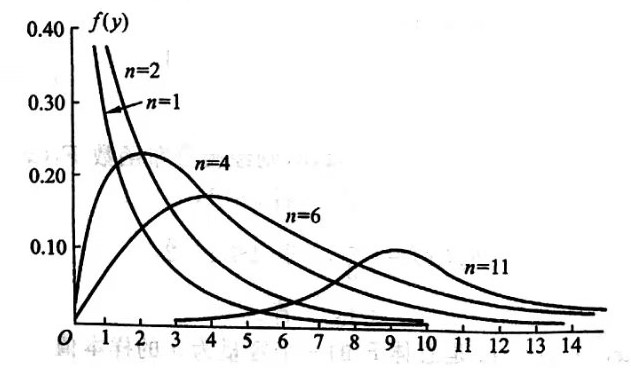
\includegraphics[scale=0.4]{1.jpg}
        \caption{$\chi^2(n)$分布的概率密度图}
    \end{figure} 
    $\chi^2(n)$分布的概率密度为
    $$f(y)=\left\{\begin{array}{ll}
        \frac{1}{2^{n/2}\Gamma (n/2)}y^{n/2-1}e^{-y/2},& y>0\\
        0,&\mbox{其他}
    \end{array}\right.$$
    $f(y)$的图形如图1所示。

\end{definition}

\begin{theorem}
    $\chi^2$分布的性质:

    {\heiti $\chi^2$分布的可加性}$\quad$ 设$\chi^2_1\sim \chi^2(n_1),\chi^2_2\sim \chi^2(n_2)$,并且
    $\chi^2_1,\chi^2_2$相互独立,则有
    $$\chi^2_1+\chi^2_2\sim \chi^2(n_1+n_2)$$

    {\heiti $\chi^2$分布的数学期望和方差}$\quad$ 若$\chi^2\sim \chi^2(n)$,则有
    $$E(\chi^2)=n,\quad D(\chi^2)=2n$$
    
    {\heiti $\chi^2$分布的上分位点}$\quad$ 对于给定的正数$\alpha,0<\alpha<1$,满足条件
    $$P\{\chi^2>\chi_\alpha^2(n)\}=\int_{\chi_\alpha^2(n)}^\infty f(y)\,dy=\alpha$$
    的点$\chi_\alpha^2(n)$就是$\chi^2(n)$分布的上$\alpha$分位点。


\end{theorem}
\clearpage
\section{参数估计}
\subsection{点估计}

\begin{definition}
    点估计问题的一般提法如下:设总体$X$的分布函数$F(x;\theta)$的形式为已知,$\theta$是待估
    参数.$X_1,X_2,\cdots,X_n$是$X$的一个样本,$x_1,x_2,\cdots,x_n$是相应的一个样本值.
    点估计问题就是要构造一个适当的统计量$\hat{\theta}(X_1,X_2,\cdots,X_n)$,用它的观察值
    $\hat{\theta}(x_1,x_2,\cdots,x_n)$作为未知参数$\theta$的近似值。称$\hat{\theta}(X_1,X_2,\cdots,X_n)$
    为$\theta$的{\heiti 估计量},称$\hat{\theta}(x_1,x_2,\cdots,x_n)$为$\theta$的{\heiti 估计值}。
    在不致混淆的情况下统称估计量和估计值为{\heiti 估计}.
\end{definition}

\begin{definition}[矩估计法]
    设$X$为连续型随机变量,其概率密度为$f(x;\theta_1,\theta_2,\cdots,\theta_k)$,或$X$为离散型随机变量,
    其分布律为$P\{X=x\}=p(x;\theta_1,\theta_2,\cdots,\theta_k)$,其中$\theta_1,\theta_2,\cdots,\theta_k$
    为待估参数,$X_1,X_2,\cdots,X_n$是来自$X$的样本.假设总体$X$的前$k$阶矩
    $$\mu_l=E(X^l)=\int_{-\infty}^\infty x^lf(x;\theta_1,\theta_2,\cdots,\theta_k)\,dx\quad X\mbox{为连续型}$$
    或
    $$\mu_l=E(X^l)=\sum_{x\in R_X}x^lp(x;\theta_1,\theta_2,\cdots,\theta_k)\quad X\mbox{为离散型}$$
    ($l=1,2,\cdots,k$,其中$R_X$是$X$可能取值的范围)存在。一般来说,它们是$\theta_1,\theta_2,\cdots,\theta_k$
    的函数.基于样本矩
    $$A_l=\frac{1}{n}\sum_{i=1}^nX_i^l$$
    依概率收敛于相应的总体矩$\mu_l(l=1,2,\cdots,k)$,样本矩的连续函数依概率收敛于相应的总体矩的连续函数,我们就用样本矩
    作为相应的总体矩的估计量,而以样本矩的连续函数作为相应的总体矩的连续函数的估计量。这种估计方法称为{\heiti 矩估计法}。

    矩估计法的具体做法如下:设
    $$\left\{\begin{array}{l}
        \mu_1=\mu_1(\theta_1,\theta_2,\cdots,\theta_k),\\
        \mu_2=\mu_2(\theta_1,\theta_2,\cdots,\theta_k),\\
        \vdots\\
        \mu_k=\mu_k(\theta_1,\theta_2,\cdots,\theta_k),\\
    \end{array}\right.$$
    这是一个包含$k$个未知参数$\theta_1,\theta_2,\cdots,\theta_k$的联立方程组。一般来说,可以从中解出$\theta_1,\theta_2,\cdots,\theta_k$,
    得到
    $$\left\{\begin{array}{l}
        \theta_1=\theta_1(\mu_1,\mu_2,\cdots,\mu_k),\\
        \theta_2=\theta_2(\mu_1,\mu_2,\cdots,\mu_k),\\
        \vdots\\
        \theta_k=\theta_k(\mu_1,\mu_2,\cdots,\mu_k),\\
    \end{array}\right.$$
    以$A_i$分别代替上式中的$\mu_i,i=1,2,\cdots,k$,就以
    $$\hat{\theta}_i=\theta_i(A_1,A_2,\cdots,A_k),i=1,2,\cdots,k$$
    分别作为$\theta_i,i=1,2,\cdots,k$的估计量,这种估计量称为{\heiti 矩估计量},矩估计量的观察值称为{\heiti 矩估计值}.
\end{definition}

\begin{definition}[最大似然估计法]
    若总体$X$属离散型,其分布律$P\{X=x\}=p(x;\theta),\theta\in \varTheta$的形式为已知,$\theta$为待估参数,$\varTheta$
    是$\theta$可能取值的范围.设$X_1,X_2,\cdots,X_n$是来自$X$的样本,则$X_1,X_2,\cdots,X_n$的联合分布律为
    $$\prod_{i=1}^np(x_i;\theta)$$
    又设$x_1,x_2,\cdots,x_n$是相应于样本$X_1,X_2,\cdots,X_n$的一个样本值.易知样本$X_1,X_2,\cdots,X_n$取到
    观察值$x_1,x_2,\cdots,x_n$的概率,亦即事件$\{X_1=x_1,X_2=x_2,\cdots,X_n=x_n\}$发生的概率为
    $$L(\theta)=L(x_1,x_2,\cdots,x_n;\theta)=\prod_{i=1}^np(x_i;\theta),\theta\in\varTheta$$
    这一概率随$\theta$的取值而变化,它是$\theta$的函数,$L(\theta)$称为样本的{\heiti 似然函数}。
    (注意,这里$x_1,x_2,\cdots,x_n$是已知的样本值,它们都是常数).

    由费希尔引进的最大似然估计法,就是固定样本观察值$x_1,x_2,\cdots,x_n$,在$\theta$取值的可能范围$\varTheta$内挑选使似然函数
    $L(x_1,x_2,\cdots,x_n;\theta)$达到最大的参数值$\hat{\theta}$,作为参数$\theta$的估计值.即取$\hat{\theta}$使
    $$L(x_1,x_2,\cdots,x_n;\hat{\theta})=\max\limits_{\theta\in\varTheta}L(x_1,x_2,\cdots,x_n;\theta)$$
    这样得到的$\hat{\theta}$与样本值$x_1,x_2,\cdots,x_n$有关,常记为$\hat{\theta}(x_1,x_2,\cdots,x_n)$,称为参数$\theta$
    的{\heiti 最大似然估计值},而相应的统计量$\hat{\theta}(X_1,X_2,\cdots,X_n)$称为参数$\theta$的{\heiti 最大似然估计量}.

    若总体$X$属连续型,其概率密度$f(x;\theta),\theta\in\varTheta$的形式已知,$\theta$为待估参数,$\varTheta$是$\theta$
    可能取值的范围.设$X_1,X_2,\cdots,X_n$是来自$X$的样本,则$X_1,X_2,\cdots,X_n$的联合密度为
    $$\prod_{i=1}^nf(x_i,\theta)$$
    设$x_1,x_2,\cdots,x_n$是相应于样本$X_1,X_2,\cdots,X_n$的一个样本值,则随机点$(X_1,X_2,\cdots,X_n)$落在点
    $(x_1,x_2,\cdots,x_n)$的邻域(边长分别为    $\,dx_1,\,dx_2,\cdots,\,dx_n$的$n$维立方体)内的概率近似地为
    \begin{equation}\tag{1}\label{7.1}
    \prod_{i=1}^nf(x_i;\theta)\,dx_i
    \end{equation}
    其值随$\theta$的取值而变化。与离散型的情况一样,取$\theta$的估计值$\hat{\theta}$使概率\eqref{7.1}取到最大值,但因子
    $\displaystyle{\prod_{i=1}^n\,dx_i}$不随$\theta$而变,故只考虑函数
    $$L(\theta)=L(x_1,x_2,\cdots,x_n;\theta)=\prod_{i=1}^nf(x_i;\theta)$$
    的最大值.这里$L(\theta)$称为样本的{\heiti 似然函数}.若
    $$L(x_1,x_2,\cdots,x_n;\hat{\theta})=\max\limits_{\theta\in \varTheta}L(x_1,x_2,\cdots,x_n;\theta)$$
    则称$\hat{\theta}(x_1,x_2,\cdots,x_n)$为$\theta$的{\heiti 最大似然估计值},称$\hat{\theta}(X_1,X_2,\cdots,X_n)$为
    $\theta$的{\heiti 最大似然估计量}。
    
    这样,确定最大似然估计量的问题就归结为微分学中的求最大值的问题了。

    在很多情况下,$p(x;\theta)$和$f(x;\theta)$关于$\theta$可微,这时$\hat{\theta}$常可从方程
    $$\frac{d}{d\theta}L(\theta)=0$$
    解得.又因$L(\theta)$和$\ln L(\theta)$在同一$\theta$处取到极值,因此,$\theta$的最大似然估计$\theta$也可以从方程
    \begin{equation}\tag{2}\label{7.2}
    \frac{d}{d\theta} \ln L(\theta)=0
    \end{equation}
    求得,而从后一方程求解往往比较方便。\eqref{7.2}称为{\heiti 对数似然方程}。

    最大似然估计法也适用于分布中含多个未知参数$\theta_1,\theta_2,\cdots,\theta_k$的情况。这时,似然函数$L$是这些未知参数的函数.
    分别令
    $$\frac{\partial}{\partial \theta_i}L=0,i=1,2,\cdots,k$$
    或令
    \begin{equation}\tag{3}\label{7.3}
    \frac{\partial}{\partial \theta_i}\ln L=0,i=1,2,\cdots,k
    \end{equation}
    解上述由$k$个方程组成的方程组,即可得到各未知参数$\theta_i(i=1,2,\cdots,k)$的最大似然估计值$\hat{\theta}_i$.
    \eqref{7.3}称为{\heiti 对数似然方程组}。
\end{definition}

\begin{theorem}
    最大似然估计具有下述性质:设$\theta$的函数$u=u(\theta),\theta\in \varTheta$具有单值反函数$\theta=\theta(u),u\in \mathfrak{U}$。又假设
    $\hat{\theta}$是$X$的概率分布中参数$\theta$的最大似然估计,则$\hat{u}=u(\hat{\theta})$是$u(\theta)$的最大似然估计。这一性质称为最大似然估计的{\heiti 不变性}.

    事实上,因为$\hat{\theta}$是$\theta$的最大似然估计,于是有
    $$L(x_1,x_2,\cdots,x_n;\theta)=\max\limits_{\theta\in \varTheta}L(x_1,x_2,\cdots,x_n,\theta)$$
    其中$x_1,x_2,\cdots,x_n$是$X$的一个样本值,考虑到$\hat{u}=u(\hat{\theta})$,且有$\hat{\theta}=\theta(\hat{u})$,上式可写成
    $$L(x_1,x_2,\cdots,x_n;\theta(\hat{u}))=\max\limits_{u\in \mathfrak{U}}L(x_1,x_2,\cdots,x_n;\theta(u))$$
    这就证明了$\hat{u}=u(\hat{\theta})$是$u(\theta)$的最大似然估计。

    当总体分布含有多个未知参数时,也具有上述性质。例如$\sigma^2$的最大似然估计为
    $$\hat{\sigma^2}=\frac{1}{n}\sum_{i=1}^n{(X_i-\overline{X})}^2$$
    函数$u=u(\sigma^2)=\sqrt{\sigma^2}$有单值反函数$\sigma^2=u^2(u\geq 0)$,根据上述性质,得到标准差$\sigma$的最大似然估计为
    $$\hat{\sigma}=\sqrt{\hat{\sigma^2}}=\sqrt{\frac{1}{n}\sum_{i=1}^n{(X_i-\overline{X})}^2}$$
\end{theorem}

\subsection{估计量的评选标准}
\begin{definition}[无偏性]
    若估计量$\hat{\theta}=\hat{\theta}(X_1,X_2,\cdots,X_n)$的数学期望$E(\hat{\theta})$存在,且对于任意$\theta\in \varTheta$有
    $$E(\hat{\theta})=\theta$$
    则称$\hat{\theta}$是$\theta$的{\heiti 无偏估计量}。
\end{definition}

\begin{definition}[有效性]
    设$\hat{\theta}_1=\hat{\theta}_1(X_1,X_2,\cdots,X_n)$与$\hat{\theta}_2=\hat{\theta}_2(X_1,X_2,\cdots,X_n)$都是
    $\theta$的无偏估计量,若对于任意$\theta\in \varTheta$,有
    $$D(\hat{\theta}_1)\leq D(\hat{\theta}_2)$$
    且至少对于某一个$\theta\in \varTheta$上式中的不等号成立,则称$\hat{\theta}_1$较$\hat{\theta}_2${\heiti 有效}。
\end{definition}

\begin{definition}[相合性]
    设$\hat{\theta}(X_1,X_2,\cdots,X_n)$为参数$\theta$的估计量,
    若对于任意$\theta\in \varTheta$,当$n \to \infty$时$\hat{\theta}(X_1,\\X_2,\cdots,X_n)$
    依概率收敛于$\theta$,则称$\hat{\theta}$为$\theta$的{\heiti 相合估计量}。

    即,若对任意$\theta\in \varTheta$都满足:对任意$\varepsilon>0$,有
    $$\lim_{n\to\infty} P\{|\hat{\theta}-\theta|<\varepsilon\}=1$$
    则称$\hat{\theta}$是$\theta$的{\heiti 相合估计量}。
\end{definition}

\subsection{区间估计}
\begin{definition}[置信区间]
    设总体$X$的分布函数$F(x;\theta)$含有一个未知参数$\theta,\theta\in \varTheta$($\varTheta$是$\theta$可能取值的范围),对于
    给定值$\alpha(0<\alpha<1)$,若由来自$X$的样本$X_1,X_2,\cdots,X_n$确定的两个统计量$\underline{\theta}=\underline{\theta}(X_1,X_2,\cdots,X_n)$
    和$\overline{\theta}=\overline{\theta}(X_1,X_2,\cdots,X_n)(\theta<\overline{\theta})$,对于任意$\theta\in\varTheta$满足
    $$P\{\underline{\theta}(X_1,X_2,\cdots,X_n)<\theta<\overline{\theta}(X_1,X_2,\cdots,X_n)\}\geq 1-\alpha$$
    则称随机区间$(\underline{\theta},\overline{\theta})$是$\theta$的置信水平为$1-\alpha$的{\heiti 置信区间},$\underline{\theta}$和$\overline{\theta}$分别称为
    置信水平为$1-\alpha$的双侧置信区间的{\heiti 置信下限}和{\heiti 置信上限},$1-\alpha$称为{\heiti 置信水平}。

    当$X$时离散型随机变量时,对于给定的$\alpha$,常常找不到区间$(\underline{\theta},\overline{\theta})$使得$P\{\underline{\theta}<\theta<\overline{\theta}\}$恰为
    $1-\alpha$。此时去找区间$(\underline{\theta},\overline{\theta})$使得$P\{\underline{\theta}<\theta<\overline{\theta}\}$至少为$1-\alpha$,且尽可能地接近$1-\alpha$.
\end{definition}

\begin{theorem}
    寻求未知参数$\theta$的置信区间的具体做法:
    \begin{enumerate}[1°]
        \item 寻求一个样本$X_1,X_2,\cdots,X_n$和$\theta$的函数$W=W(X_1,X_2,\cdots,X_n;\theta)$,使得$W$的分布不依赖于
        $\theta$以及其他未知参数,称具有这种性质的函数$W$为{\heiti 枢轴量}.
        \item 对于给定的置信水平$1-\alpha$,定出两个常数$a,b$,使得
        $$P\{a<W(X_1,X_2,\cdots,X_n;\theta)<b\}=1-\alpha$$
        若能从$a<W(X_1,X_2,\cdots,X_n;\theta)<b$得到与之等价的$\theta$的不等式$\underline{\theta}<\theta<\overline{\theta}$,其中
        $\underline{\theta}=\underline{\theta}(X_1,X_2,\cdots,X_n),\overline{\theta}=\overline{\theta}(X_1,X_2,\cdots,X_n)$都是统计量。
        那么$(\underline{\theta},\overline{\theta})$就是$\theta$的一个置信水平为$1-\alpha$的置信区间。
    \end{enumerate}
    
    枢轴量$W(X_1,X_2,\cdots,X_n;\theta)$的构造,通常可以从$\theta$的点估计着手考虑。常用的正态总体的参数的置信区间可以用上述步骤推得。
\end{theorem}

\subsection{正态总体均值与方差的区间估计}
\begin{theorem}
    设已给定置信水平为$1-\alpha$,并设$X_1,X_2,\cdots,X_n$为总体$N(\mu,\sigma^2)$的样本。$\overline{X},S^2$分别是样本均值和样本方差。
    \begin{enumerate}[1.]
        \item 均值为$\mu$的置信区间
        \begin{enumerate}[(1)]
            \item $\sigma^2$为已知,可得$\mu$的一个置信水平为$1-\alpha$的置信区间为
            $$(\overline{X}\pm \frac{\sigma}{\sqrt{n}}z_{\alpha/2})$$
            \item $\sigma^2$为未知,可得$\mu$的一个置信水平为$1-\alpha$的置信区间为
            $$(\overline{X}\pm \frac{S}{\sqrt{n}}t_{\alpha/2}(n-1))$$
        \end{enumerate}
        \item 方差$\sigma^2$的置信区间
            
        方差$\sigma^2$的一个置信水平为$1-\alpha$的置信区间为
        $$\left(\frac{(n-1)S^2}{\chi ^2_{\alpha/2}(n-1)},\frac{(n-1)S^2}{\chi^2_{1-\alpha/2}(n-1)}\right)$$
        标准差$\sigma$的一个置信水平为$1-\alpha$的置信区间为
        $$\left(\frac{\sqrt{n-1}S}{\sqrt{\chi ^2_{\alpha/2}(n-1)}},\frac{\sqrt{n-1}S}{\sqrt{\chi^2_{1-\alpha/2}(n-1)}}\right)$$
    \end{enumerate}        
\end{theorem}

\begin{theorem}
    设已给定置信水平为$1-\alpha$,并设$X_1,X_,2,\cdots,X_{n_1}$是来自第一个总体的样本;$Y_1,Y_2,\cdots,Y_{n_2}$是来自第二个
    总体的样本,这两个样本相互独立。且设$\overline{X},\overline{Y}$分别为第一、第二个总体的样本均值,$S_1^2,S_2^2$分别是第一、第二个
    总体的样本方差。
    \begin{enumerate}[1.]
        \item 两个总体均值差$\mu_1-\mu_2$的置信区间
        \begin{enumerate}[(1)]
            \item $\sigma_1^2,\sigma_2^2$均为已知,$\mu_1-\mu_2$的一个置信水平为$1-\alpha$的置信区间$$\left(\overline{X}-\overline{Y}\pm z_{\alpha/2}\sqrt{\frac{\sigma_1^2}{n_1}+\frac{\sigma^2_2}{n_2}}\right)$$
            \item $\sigma_1^2=\sigma_2^2=\sigma^2$,但$\sigma^2$未知,此时$\mu_1-\mu_2$的一个置信水平为$1-\alpha$的置信区间为
            $$\left(\overline{X}-\overline{Y}\pm t_{\alpha/2}(n_1+n_2-2)S_w\sqrt{\frac{1}{n_1}+\frac{1}{n_2}}\right)$$
            此处$\displaystyle{S_w^2=\frac{(n_1-1)S_1^2+(n_2-1)S_2^2}{n_1+n_2-2},S_w=\sqrt{S_w^2}}$
        \end{enumerate}
        \item 两个总体方差比$\sigma_1^2/\sigma_2^2$的置信区间
        
        对于总体均值$\mu_1,\mu_2$均为未知时,$\sigma_1^2/\sigma_2^2$的一个置信水平为$1-\alpha$的置信区间为
        $$\left(\frac{S_1^2}{S_2^2}\frac{1}{F_{\alpha/2}(n_1-1,n_2-1)},\frac{S_1^2}{S_2^2}\frac{1}{F_{1-\alpha/2}(n_1-1,n_2-1)}\right)$$
    \end{enumerate} 
\end{theorem}

\subsection{(0-1)分布参数的区间估计}
    \begin{theorem}
        已知$(0-1)$分布的均值和方差分别为$$\mu=p,\sigma^2=p(1-p)$$
        设$X_1,X_2,\cdots,X_n$是一个样本,因样本容量$n$比较大,由中心极限定理,知
        $$\frac{\sum\limits_{i=1}^n X_i-np}{\sqrt{np(1-p)}}=\frac{n\overline{X}-np}{\sqrt{np(1-p)}}$$
        近似地服从$N(0,1)$分布,于是有
        $$P\left\{-z_{\alpha/2}<\frac{n\overline{X}-np}{\sqrt{np(1-p)}}<z_{\alpha/2}\right\}\approx 1-\alpha$$
        而不等式
        \begin{equation}\tag{4}\label{7.6}
            -z_{\alpha/2}<\frac{n\overline{X}-np}{\sqrt{np(1-p)}}<z_{\alpha/2}
        \end{equation}
        等价于
        $$(n+z^2_{\alpha/2})p^2-(2n\overline{X}+z^2_{\alpha/2})p+n\overline{X}^2<0$$
        记$$p_1=\frac{1}{2a}(-b-\sqrt{b^2-4ac})$$
        $$p_2=\frac{1}{2a}(-b+\sqrt{b^2-4ac})$$
        此处$a=n+z^2_{\alpha/2},b=-(2n\overline{X}+z^2_{\alpha/2}),c=n\overline{X}^2$。于是由\eqref{7.6}式得$p$的一个近似的置信水平为$1-\alpha$的置信区间为
        $$(p_1,p_2)$$
    \end{theorem}
 
\subsection{单侧置信区间}
    \begin{definition}
        对于给定值$\alpha(0<\alpha<1)$,若由样本$X_1,X_2,\cdots,X_n$确定的统计量$\underline{\theta}=\underline{\theta}(X_1,X_2,\cdots,X_n)$,对于任意$\theta\in \varTheta$满足
        $$P\{\theta>\underline{\theta}\}\geq 1-\alpha$$
        称随机区间$(\underline{\theta},\infty)$是$\theta$的置信水平为$1-\alpha$的{\heiti 单侧置信区间},$\underline{\theta}$称为$\theta$的置信水平为$1-\alpha$的{\heiti 单侧置信下限}。

        又若统计量$\overline{\theta}=\overline{\theta}(X_1,X_2,\cdots,X_n)$,对于任意$\theta\in \varTheta$满足
        $$P\{\theta<\overline{\theta}\}\geq 1-\alpha$$
        称随机区间$(-\infty,\overline{\theta})$是$\theta$的置信水平为$1-\alpha$的{\heiti 单侧置信区间},$\overline{\theta}$称为$\theta$的置信水平为$1-\alpha$的{\heiti 单侧置信上限}。

        例如对于正态总体$X$,若均值$\mu$,方差$\sigma^2$均为未知,设$X_1,X_2,\cdots,X_n$是一个样本,由
        $$\frac{\overline{X}-\mu}{S/\sqrt{n}}\sim t(n-1)$$
        有$$P\left\{\frac{\overline{X}-\mu}{S/\sqrt{n}}<t_\alpha(n-1)\right\}=1-\alpha$$
        即$$P\left\{\mu>\overline{X}-\frac{S}{\sqrt{n}}t_\alpha(n-1)\right\}=1-\alpha$$
        于是得到$\mu$的置信水平为$1-\alpha$的单侧置信区间
        $$\left(\overline{X}-\frac{S}{\sqrt{n}}t_\alpha(n-1),\infty\right)$$
        $\mu$的置信水平为$1-\alpha$的单侧置信下限为
        $$\underline{\mu}=\overline{X}-\frac{S}{\sqrt{n}}t_\alpha(n-1)$$
        又由$$\frac{(n-1)S^2}{\sigma^2}\sim \chi^2(n-1)$$
        有
        $$P\left\{\frac{(n-1)S^2}{\sigma^2}>\chi_{1-\alpha}^2(n-1)\right\}=1-\alpha$$
        即
        $$P\left\{\sigma^2<\frac{(n-1)S^2}{\chi_{1-\alpha}^2(n-1)}\right\}=1-\alpha$$
        于是得$\sigma^2$的置信水平为$1-\alpha$的单侧置信区间
        $$\left(0,\frac{(n-1)S^2}{\chi_{1-\alpha}^2(n-1)}\right)$$
        $\sigma^2$的置信水平为$1-\alpha$的单侧置信上限为
        $$\overline{\sigma^2}=\frac{(n-1)S^2}{\chi_{1-\alpha}^2(n-1)}$$
    \end{definition}

    
\clearpage
\section{假设检验}
\subsection{假设检验}
\clearpage
\section{方差分析及回归分析}
\subsection{单因素试验的方差分析}
\end{document}
